%!TEX TS-program = lualatex
%!TEX encoding = UTF-8 Unicode

\documentclass{beamer}

\usepackage{fontspec}
\newfontfamily{\FAFR}{FontAwesome}
\usepackage{polyglossia}
\setdefaultlanguage{english}
\setotherlanguage{swedish}
\usepackage[english]{selnolig}

\usepackage{csquotes}
\usepackage{microtype}
\usepackage{booktabs}
\usepackage{colortbl}
\usepackage{multirow}
\usepackage{array}

%\usepackage{beamerthemesplit}

%\usepackage{pdfpages}
%\usepackage[natbib=true,citestyle=numeric]{biblatex}
%\usepackage{rotating}

%\usepackage{tikz}
%\usetikzlibrary{shapes}
%\usetikzlibrary {positioning}
%\definecolor {processblue}{cmyk}{0.96,0,0,0}

\usepackage{graphicx}
\usepackage{minted}

\usenavigationsymbolstemplate{}
%\usetheme{Luebeck}
\usetheme{metropolis}

%\usepackage{beamerthemeIntel}
\setbeamercolor{background canvas}{bg=}	% required for includepdf

%\bibliography{../paper/reflist.bib}

\title[Running Linux kernel filesystem drivers in userspace using Linux Kernel Library (LKL)]{Running Linux kernel filesystem drivers in userspace using Linux Kernel Library (LKL)}
\subtitle{}
\author{Andreas Gnau}
\date{\today}

% BEGIN: speaker notes on the right (comment to hide notes)
% can be comfortably views with dspdfviewer (Linux)
% ==> seems to work on Mac as well, but needs to be compiled
% or Skim (Mac) http://skim-app.sourceforge.net/
%\def\shownotesright{}
\ifdefined\shownotesright
\usepackage{pgfpages}
\setbeameroption{show notes}
\setbeameroption{show notes on second screen=right}
\else\ifdefined\shownotesonly
\setbeameroption{show only notes}
\fi
\fi

% END: speaker notes on the right


\usepackage{hyperref}
\hypersetup{pdfusetitle, colorlinks=false, hidelinks}
% pdfpagemode=FullScreen


% uncomment below (and comment above) to print the notes only
%\setbeameroption{show only notes}

\begin{document}

    %!TEX TS-program = xelatex
%!TEX encoding = UTF-8 Unicode

%\frame[plain]{ % When including a large figure or table, you don't want to have the bottom and the top of the slides.
%\frame[shrink]{ % If you want to include lots of text on a slide, use the shrink option.

% Explain why we did this research
\frame[plain]{
\titlepage
\note{
    \begin{itemize}
%        \item probably wondered why I sound so strange when speaking Swedish
%        \item German
%        \item I have been consultant for software after my bachelor's
%        \item after three years, decided to get adventurous and study in Sweden 
        \item My name is Andreas Gnau.
        \item work at Sylog a consultant company and Embedded Linux is what I am mostly dealing with.
        \item and today I will tell you about a project called Linux Kernel Library
        \item and how it can be used to re-use Linux-kernel fs drivers
        \item run in user space
    \end{itemize}
}

}


%    \section[Outline]{}
        \frame{
             \frametitle{Outline}
            \tableofcontents \note{
        \begin{itemize}
            \item \textbf{first start} with a motivation on why one would want do that...
            \item \textbf{followed by }background information on the different technologies
            \item \textbf{Then I will continue to} briefly present some performance numbers
            \item \textbf{After that } I will summarize about applications of LKL in the FS domain and other domains
            \item and finish my talk with future work
        \end{itemize}
    }}
    \section{Motivation}
        %!TEX TS-program = lualatex
%!TEX encoding = UTF-8 Unicode

%\frame[plain]{ % When including a large figure or table, you don't want to have the bottom and the top of the slides.
%\frame[shrink]{ % If you want to include lots of text on a slide, use the shrink option.

\begin{frame}
    
    \frametitle{Motivation}
    
    File systems are complex code bases (ext4:~50~KLOC)
    
    Security bugs are a risk, because most file systems run in kernel space.
    
    
    
    \note{
        \begin{itemize}
            \item Everyone uses FS
            \item lot of features, journaling, snapshots, raid, encryption
            \item ext4 50 KLOC, btrfs: 130KLOC
            \item security bugs (and other bugs) are a risk
            \item run in kernel space, i.e. with highest privileges
            \item code execution there, game over. 
        \end{itemize}
    }
\end{frame}
        %%!TEX TS-program = lualatex
%!TEX encoding = UTF-8 Unicode

%\frame[plain]{ % When including a large figure or table, you don't want to have the bottom and the top of the slides.
%\frame[shrink]{ % If you want to include lots of text on a slide, use the shrink option.

\begin{frame}

    \frametitle{Demo Time!}
    
    Demo: Let's connect that USB drive...

    \note{
        \begin{itemize}
            \item Pray to the demo gods...
            \item So this is blue light, and a USB cable, leading to a separate machine
            \item When I was 15, I thought it was a good idea to spend my pocket money on USB-cables with blue light.
            \item I realised that it is not very useful investment well I before I turned 16, so don't buy them
            \item Anyways... So I will connect this USB drive...
            \item NP deref, could be use-after-free, out-of-bounds-write...
            
        \end{itemize}
    }
\end{frame}
        %!TEX TS-program = lualatex
%!TEX encoding = UTF-8 Unicode

%\frame[plain]{ % When including a large figure or table, you don't want to have the bottom and the top of the slides.
%\frame[shrink]{ % If you want to include lots of text on a slide, use the shrink option.

\begin{frame}

    \frametitle{Is it a big problem?}
    
        \begin{itemize}
            \item<2-> It depends...
            \item<3-> There are easier ways: downloading and executing files via a browser, BadUSB...
        \end{itemize}
    
        \only<4->{... but...}

        \begin{itemize}
            \item<4-> Unattended PC with lock screen
            \item<4-> Connecting untrusted USB disks
            \item<4-> Air-Gapped machines
            \item<4-> Double-clicking filesystem images (depends on configuration)
        \end{itemize}
    \note{
        \begin{itemize}
            \item \textbf{Ask: So, who thinks this is a big prob, who doesn't, why?}
            \item It depends...
            \item There are easier ways: downloading and executing files via a browser, BadUSB...
            \item Unattended PC with lock screen
            \item Connecting USB disks
            \item Double-clicking filesystem images (depends on configuration)
            \item Air-Gapped machines
            
        \end{itemize}
    }
\end{frame}

    \section{Background}
        %!TEX TS-program = lualatex
%!TEX encoding = UTF-8 Unicode

%\frame[plain]{ % When including a large figure or table, you don't want to have the bottom and the top of the slides.
%\frame[shrink]{ % If you want to include lots of text on a slide, use the shrink option.

\begin{frame}
    \frametitle{FUSE (File System in User Space)}
    \begin{center}
        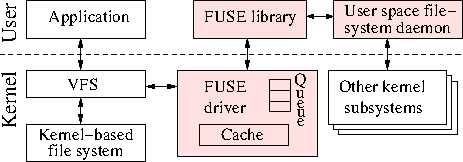
\includegraphics[width=.7\textwidth]{frames/img/fuse_arch}
    \end{center}
    
    \begin{itemize}
        \item simplifies writing file system drivers by avoiding kernel-level code
        \item mounting / unmounting can be done as an unprivileged user
        \item file ownership can be adjusted to enable unprivileged access to the filesystem
    \end{itemize}
    
    \note{
    \begin{itemize}
        \item kernel driver exposes a queue of requests to user space...
        \item ... which is consumed by a user space daemon handling those requests
        \item Of course there is some overhead due to context switches and copying
        \item simplifies writing file system drivers by avoiding kernel-level code
        \item mounting / unmounting can be done as a unprivileged user
        \item file ownership can be adjusted to enable unprivileged access to the filesystem
    \end{itemize}
    }
\end{frame}
        %!TEX TS-program = lualatex
%!TEX encoding = UTF-8 Unicode

%\frame[plain]{ % When including a large figure or table, you don't want to have the bottom and the top of the slides.
%\frame[shrink]{ % If you want to include lots of text on a slide, use the shrink option.

\begin{frame}
    \frametitle{libguestfs}
    \begin{itemize}
        \item library and suite of utilities for offline FS access
        \item uses a dedicated VM for filesystem access
        \item mature ecosystem, many useful CLI utilities
        \item FUSE filesystem available as well, but very slow
    \end{itemize}

\begin{center}
    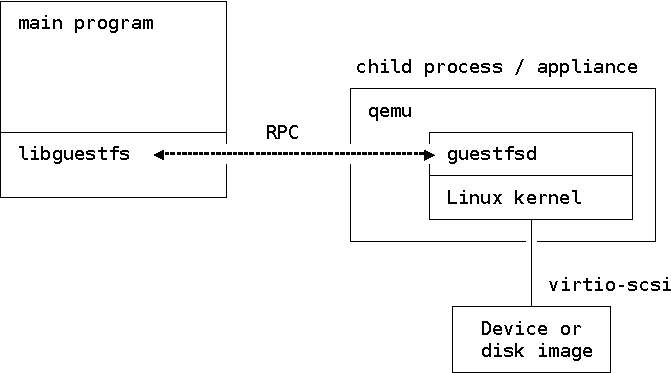
\includegraphics[width=.65\textwidth]{frames/img/libguestfs_arch}
\end{center}
    
    \note{
        \begin{itemize}
            \item \textbf{Q} library and suite of utilities for offline FS access
            \item Approach: runs a small virtual machine with  Linux that does the FS-access
            \item process on the host talks to process in the VM
            \item quite some overhead, but the goal is to isolate the operations from the host
            \item fast CLI utils, slow FUSE => additional overhead, because data is transferred in smaller chunks
        \end{itemize}
    }
\end{frame}
        %!TEX TS-program = xelatex
%!TEX encoding = UTF-8 Unicode

%\frame[plain]{ % When including a large figure or table, you don't want to have the bottom and the top of the slides.
%\frame[shrink]{ % If you want to include lots of text on a slide, use the shrink option.

\begin{frame}
    \frametitle{Linux Kernel Library (LKL)}
        \begin{columns}[c]
            \begin{column}{.45\textwidth}
                \begin{itemize}
                    \item arch-port of the Linux kernel
                    \item only basic primitives are implemented on the host side (threading, TLS, semaphores, timers...)
                    \item CLI-utilities and experimental FUSE exist
                \end{itemize}
            \end{column}
            \begin{column}{.55\textwidth}
%\includegraphics[width=.9\textwidth]{frames/img/lkl_overview}
            \end{column}
        \end{columns}


    \note{
        \begin{itemize}
            \item arch-port similiar to UML to enable use as a library
            \item interface is the syscalls, e.g. lkl\_sys\_getpid()
            \item basic primitives are implemented for each host, POSIX, Win32, Windows Kernel, Haiku OS
            \item interesting use cases EFI filesystem driver, running LKL inside a SGX enclave etc.
        \end{itemize}
    }
\end{frame}

    \section{Performance}
        %!TEX TS-program = lualatex
%!TEX encoding = UTF-8 Unicode

%\frame[plain]{ % When including a large figure or table, you don't want to have the bottom and the top of the slides.
%\frame[shrink]{ % If you want to include lots of text on a slide, use the shrink option.


\begin{frame}[plain]
    \frametitle{Throughput Relative to Linux Loopback Mounting}
    \vspace*{-1pt}
    \makebox[\linewidth]{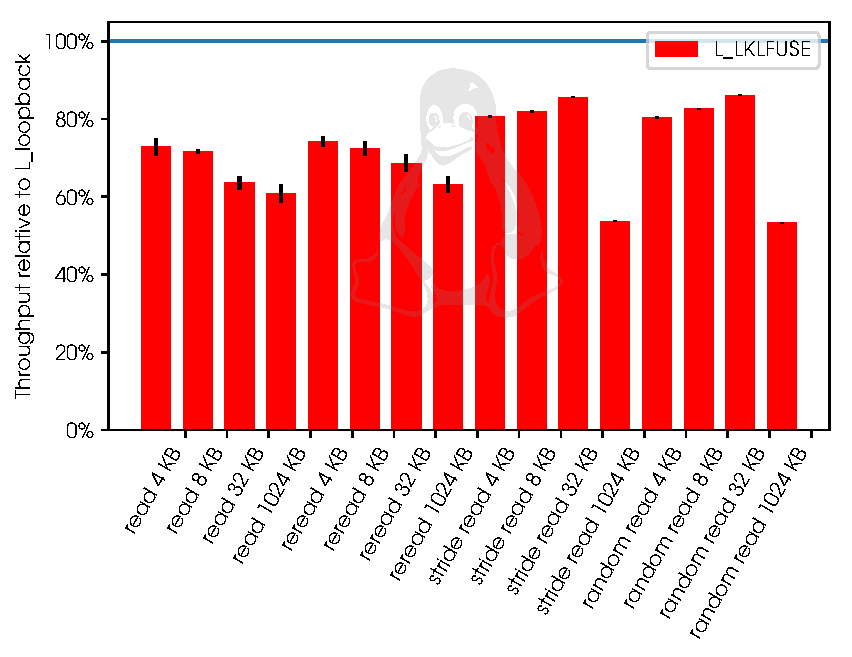
\includegraphics[page=1,width=0.87\paperwidth]{frames/img/relative_performance_filter_read_baseline_L_loopback_variants_L_LKLFUSE}}
    \note{
        \begin{itemize}
            \item blue line is baseline, mounting FS via Linux Kernel
            \item Y-access LKLFUSE relative to baseline loopback-mounting
            \item X-axis, workloads
            \item LKLFUSE delivers okay read performance, i.e. 72\%
            \item very consistent irregardless of blocksize. readahead
        \end{itemize}
    }
\end{frame}

\begin{frame}[plain]
\frametitle{Throughput Relative to Linux Loopback Mounting}
\vspace*{-1pt}
\makebox[\linewidth]{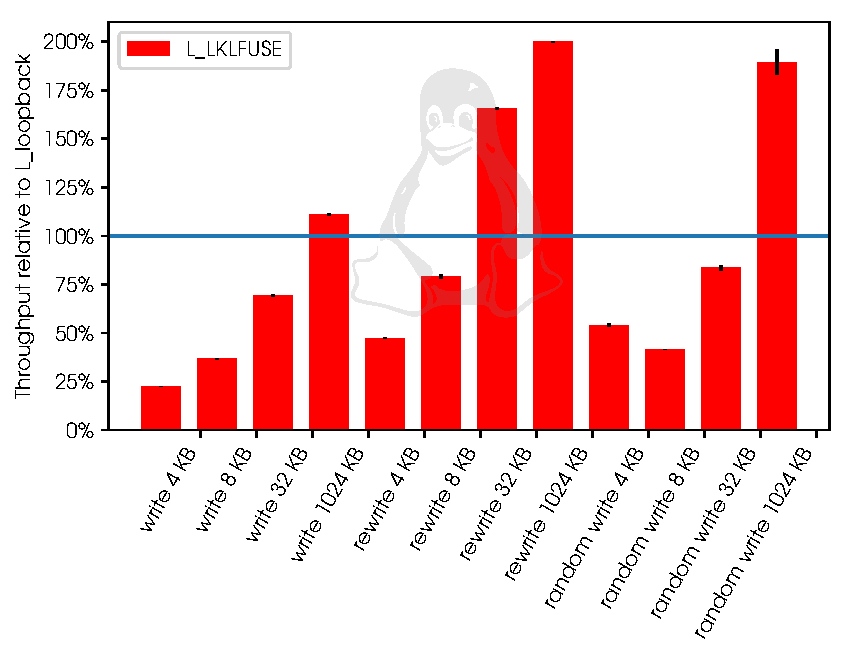
\includegraphics[page=1,width=0.87\paperwidth]{frames/img/relative_performance_filter_write_baseline_L_loopback_variants_L_LKLFUSE}}
\note{
    \begin{itemize}
        \item LKLFUSE: seq write delivers okay performance, i.e. above 50\%
        \item big difference between blocksizes. Overhead of each write reaching the FS one by one
        \item much better than baseline: how is that possible?
        \item writing to pages that have not been written back (rewrite, random write), writeback caching
        \item multiple layers of caching
    \end{itemize}
}
\end{frame}


    \section{Applications}
        %!TEX TS-program = lualatex
%!TEX encoding = UTF-8 Unicode

%\frame[plain]{ % When including a large figure or table, you don't want to have the bottom and the top of the slides.
%\frame[shrink]{ % If you want to include lots of text on a slide, use the shrink option.

\begin{frame}

    \frametitle{Applications within filesystems}
    
        \begin{itemize}
            \item Mounting filesystem images without root-access
            \item Manipulating files without mounting (CLI or library)
            \item Re-using well-tested drivers from Linux in other OSes or bootloaders
            \item Mounting untrusted filesystems (in the future, no good isolation, yet)
            \item Use LKL for mounting filesystem types with a bad security record
        \end{itemize}

    \note{
        \begin{itemize}
            \item Mounting filesystem images without root-access
            \item Manipulating files without mounting (CLI or library)
            \item Re-using well-tests drivers from Linux in other OSes or even bootloaders (FreeBSD FUSE, UEFI, Haiku OS)
            \item Mounting untrusted filesystems (no good protection, yet)
            \item Use LKL for mounting filesystem types with a bad security record
        \end{itemize}
    }
\end{frame}
        %!TEX TS-program = lualatex
%!TEX encoding = UTF-8 Unicode

%\frame[plain]{ % When including a large figure or table, you don't want to have the bottom and the top of the slides.
%\frame[shrink]{ % If you want to include lots of text on a slide, use the shrink option.

\begin{frame}

    \frametitle{Use cases}
    
        \begin{itemize}
            \item Userspace networking
            \item Network simulations
            \item Unikernels
            \item Development: use space tools are more widely-available and more mature
            \item Profiling
            \item Fuzzing
        \end{itemize}

    \note{
        \begin{itemize}
            \item Userspace networking
            \item Network simulations
            \item Unikernels
            \item Development: Use space tools are widely-available mature, easier to user
            \item Fuzzing filesystem and network stack
        \end{itemize}
    }
\end{frame}

    \section{Current Status and Future Work}
        %!TEX TS-program = lualatex
%!TEX encoding = UTF-8 Unicode

%\frame[plain]{ % When including a large figure or table, you don't want to have the bottom and the top of the slides.
%\frame[shrink]{ % If you want to include lots of text on a slide, use the shrink option.

\begin{frame}
    
    \frametitle{Current Status and Future Work}
    
    \makebox[\linewidth]{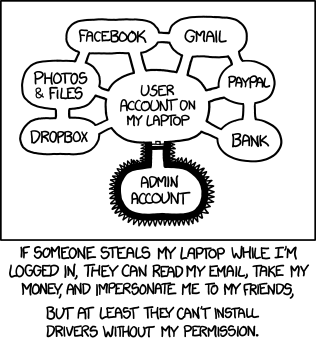
\includegraphics[width=0.57\paperwidth]{frames/img/xkcd_1200_authorization}}
    
    \note{
        \begin{itemize}
            \item lklfuse runs as user mounting the thing...
        \end{itemize}
    }
\end{frame}
        %!TEX TS-program = lualatex
%!TEX encoding = UTF-8 Unicode

%\frame[plain]{ % When including a large figure or table, you don't want to have the bottom and the top of the slides.
%\frame[shrink]{ % If you want to include lots of text on a slide, use the shrink option.

\begin{frame}

    \frametitle{Outlook on Future Work}
    
    \begin{itemize}
        \item LKLFUSE (me):
            \begin{itemize}
                \item currently working on: better performance and more correct behaviour using libfuse3  and low-level API
                \item Future: integration, running under less privileged account, maybe use seccomp-bpf...
            \end{itemize}

        \item Other developments in progress:
            \begin{itemize}
                \item Mainlining
                \item KASAN support
                \item Support for multiple processes (fork)
            \end{itemize}
        
    \end{itemize}

    \note{
        \begin{itemize}
            \item Pray to the demo gods...
            \item So this is blue light, and a USB cable, leading to a separate machine
            \item When I was 15, I thought it was a good idea to spend my pocket money on USB-cables with blue light.
            \item I realised that it is not very useful investment well I before I turned 16, so don't buy them
            \item Anyways... So I will connect this USB drive...
            \item NP deref, could be use-after-free, out-of-bounds-write...
            
        \end{itemize}
    }
\end{frame}

%    \section*{Backup Slides}
        %!TEX TS-program = xelatex
%!TEX encoding = UTF-8 Unicode

%\frame[plain]{ % When including a large figure or table, you don't want to have the bottom and the top of the slides.
%\frame[shrink]{ % If you want to include lots of text on a slide, use the shrink option.

\begin{frame}
    
    \frametitle{Thanks!}
        \begin{center}
            \huge{Questions?}
        \end{center}
    \note{
        \begin{itemize}
            \item like it here
            \item learned a lot
            \item scope was too wide, lklfuse + utils would have been enough
            \item could have asked for help more often
            \item thank everyone who made me feel welcome, gave advice, talked Swedish with me even if it was a bit of a hassle
            \item learned to work in Sweden
        \end{itemize}
         }
    
    
    
\end{frame}


\begin{frame}

\frametitle{Backup Slides}
    
\note{note text}



\end{frame}



        %%!TEX TS-program = xelatex
%!TEX encoding = UTF-8 Unicode

%\frame[plain]{ % When including a large figure or table, you don't want to have the bottom and the top of the slides.
%\frame[shrink]{ % If you want to include lots of text on a slide, use the shrink option.

% Explain why we did this research

\begin{frame}[fragile]
    \begin{listing}[H]
        \begin{minted}{console}
# losetup --find --show --partscan debian8.img
/dev/loop0

# file -s /dev/loop0*
/dev/loop0:   DOS/MBR boot sector
/dev/loop0p1: Linux rev 1.0 ext4 filesystem data, UUID=b90f0480-a8b5-4369-a2c5-31d005477b10 (extents) (large files) (huge files)
/dev/loop0p2: DOS/MBR boot sector; partition 1 : ID=0x83, start-CHS (0x17a,28,35), end-CHS (0x233,120,5), startsector 2, 2977792 sectors; partition 2 : ID=0x5, start-CHS (0x233,120,6), end-CHS (0x273,184,5), startsector 2977794, 1032192 sectors, extended partition table
/dev/loop0p5: Linux rev 1.0 ext4 filesystem data, UUID=48308279-ef74-4d5e-8c14-547d7178afa3 (extents) (large files) (huge files)
/dev/loop0p6: Linux/i386 swap file (new style), version 1 (4K pages), size 128767 pages, no label, UUID=963e44b9-9534-4a0f-8d63-5006653bf40a
/dev/loop0p7: Linux rev 1.0 ext4 filesystem data, UUID=4c5efdb6-6647-437d-99db-86f33a8ca417 (extents) (huge files)
/dev/loop0p8: Linux rev 1.0 ext4 filesystem data, UUID=d7f0d2c9-1a40-4c06-8c68-374c3ad45ee6 (needs journal recovery) (extents) (large files) (huge files)

# mount /dev/loop0p5 /mnt/mountpoint
        \end{minted}
    
        \caption{Recent versions of util-linux allow creating loop-devices for individual partitions}

        \label{lst:mount_loop}
    \end{listing}
    
\note{
    \begin{itemize}
        \item Mounting images without partition table (filesystem images)% \mintinline{console}{# mount -o loop img /mnt} works fine}
        \item If the loop-/sys/module/loop/parameters/max\_part
        \item Older versions of util-linux do not support the --partscan-parameter which will instruct the kernel to read the partition table. The partprobe-command from libparted can be a replacement in this case. On kernels older than 3.2, the loop module has to be loaded with a non-zero max\_part parameter.
        https://git.kernel.org/cgit/utils/util-linux/util-linux.git/commit/?id=59d749c33136b85fc4a51a0af6c48cc97e3d1b31
    \end{itemize}
}



\end{frame}



        
    
%	\input{frames/references.tex}
\end{document}